\documentclass[a4paper]{article}

%% Language and font encodings


%% Sets page size and margins
\usepackage[a4paper,top=3cm,bottom=2cm,left=3cm,right=3cm,marginparwidth=1.75cm]{geometry}

%% Useful packages
\usepackage{amsmath,amssymb,bm}
\usepackage{graphicx,multirow,tabularx}
\usepackage[colorlinks=true, allcolors=blue]{hyperref}

\usepackage{tikz}
\usetikzlibrary{positioning,fit,bayesnet}
\tikzset{
latent/.style={circle, minimum size = 12mm, thick, draw =black!100, node distance = 12mm},
observed/.style={circle, minimum size = 12mm, thick, draw =black!100, fill=black!20, node distance = 12mm},
empty/.style={circle, minimum size = 12mm, thick, draw =white!100, fill=white!100, node distance = 12mm},
hyper/.style={circle, minimum size = 8mm, thick, draw =black!100, node distance = 8mm},
%plate/.style={rectangle, inner sep=4mm, draw=black!100},
connect/.style={-latex, thick}
}


\newcommand{\score}[1]{ \noindent \emph{#1 pt(s)}\\}

\newcolumntype{Y}{>{\centering\arraybackslash}X}
\renewcommand{\arraystretch}{2}
\renewcommand{\v}[1]{\mathbf{\bm #1}}
\renewcommand{\vec}[1]{\mathbf{\bm #1}}

\title{Bayesian Statistics}
\author{Exercises for week 04}
\date{\vspace{-5ex}}

\begin{document}
\maketitle


\section{Cooking with Bayesian inference}
\score{5}

In this exercise, you'll translate a `realistic' scenario into a hierarchical Bayesian model. Part of the exercise requires you to search online for function names and ways of specifying data structures in \texttt{R}. Oftentimes, you'll find that there are different ways of achieving a particular goal.

Consider the following setting. I'm making dinner according to $K=4$ different cooking shows. Let's refer to the shows as Gordon, Jamie, Julia and Nigella. Unfortunately, the quality of each tv show's recipes can differ.

\begin{itemize}
    \item I'm trying $N$ dinners.
    \item A dinner $i$ is either tasty ($x_i=1$) or a failure ($x_i=0$).
    \item Each cooking show $k$ has its own success probability $\theta$.
    \item The label $z_i \in \{1, \ldots, K\}$ indicates on which show the dinner $i$ is based.
    \item The success of the dinner depends only on the success probability $\theta$ and the label $z$.\footnote{And not on my cooking skills, obviously.}
    \item Each show has its own `pseudo-success count' $a$ and `pseudo-failure count' $b$.
    \item For every dinner, I pick a tv show uniformly at random, that is, by drawing a random tv show $z$ from a \emph{categorical} distribution with parameter $\v{\alpha}=1/K \times \v{1}_K$, where $\v{1}_K$ means a vector of length $K$ containing only ones (i.e. each show is equally likely in the prior).
\end{itemize}

Construct the model:

\begin{enumerate}
    \item The first step in modeling this scenario is to draw a graphical model (using plate notation). You'll need to think about which parameters depend on which other parameters, and, conversely, which parameters are \emph{independent}, and which parameters are repeating. Also, some parameters will require subscript indices, which are not always shown in the outline above!\footnote{Tip: the \texttt{.tex} file for this exercise is also available on Blackboard. You can use it to see how I draw the diagram in the next exercise, using \texttt{Tikz}.}
    
    \item The second step is to specify by which probability distribution each of the dependencies in your model may be described. Clearly indicate the name of the distribution, what parameters go in, what parameter comes out, and any (if applicable) constraints on the outcomes. Use the \emph{generative model} notation as in the lecture (or see e.g. the next exercise).
    
    \item With your model, you can now generate $N$ simulated observations $x_1,\ldots,x_N$. Write an \texttt{R} script that does this, for $N=100$. Begin the script by setting the hyperparameters for each tv show. Using the hyperparameters, you can draw the next layer of parameters (for each..?). With those parameters, you can draw the actual observations $\v{x}$. Summarize your output as follows: show for each tv show how many dinners it has in the simulated data, and how many of these were a success. Show this output for the following three cases, and show which hyperparameter settings you used to encode the following beliefs:
        \begin{enumerate}
          \item You have strong prior beliefs (hope?) that the recipes by Jamie were a success.
          \item You think it doesn't matter in which tv show I watched; you think it'll be a failure anwyay. 
          \item You have absolutely no idea what these tv dinner shows are, so you have uniform prior beliefs about each of their success probabilities.
        \end{enumerate}
        Verify that the generated data is as you would expect for your hyperparameter settings!
\end{enumerate}

Some tips: \texttt{R} does not (by default) contain an implementation for the Categorical distribution. However, you can use the function \texttt{sample}.


\section{A 1-D Gaussian mixture model}
\score{5}

\begin{figure}[t]
    \centering
    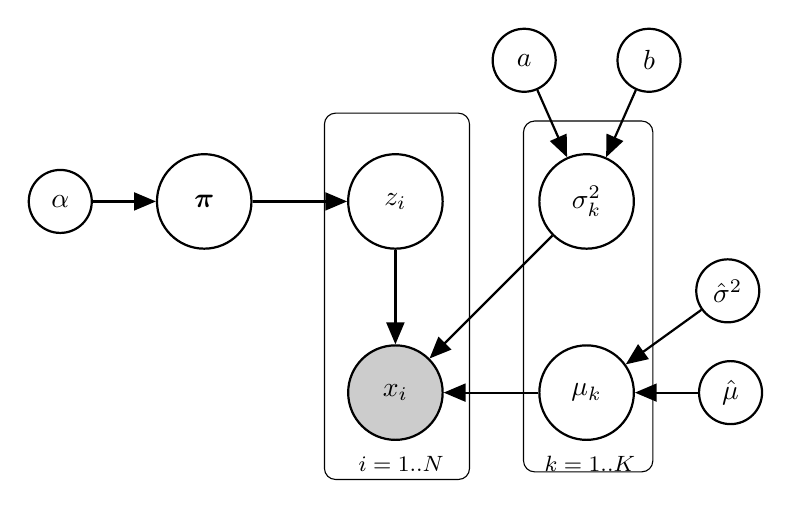
\begin{tikzpicture}
        \node[observed](xi){$x_i$};
        \node[latent, above=of xi](zi){$z_i$};
        \plate[inner sep=.3cm,xshift=.02cm,yshift=.2cm] {points} {(xi) (zi)} {$i=1..N$};
        \node[latent, left=of zi] (pi) {$\v{\pi}$};
        \node[hyper, left=of pi] (alpha) {$\alpha$};
        \node[latent, right=of xi] (mu_k) {$\mu_k$};
        \node[latent, right=of zi] (sigma_k) {$\sigma^2_k$};
        \plate[inner sep=0.2cm,xshift=.02cm,yshift=.2cm] {clusters} {(mu_k) (sigma_k)} {$k=1..K$};

        \node[hyper, above left=of sigma_k,xshift=0.5cm,yshift=0.5cm] (a) {$a$};
        \node[hyper, above right=of sigma_k,xshift=-0.5cm,yshift=0.5cm] (b) {$b$};

        \node[hyper, right=of mu_k] (mu_sup) {$\hat{\mu}$};
        \node[hyper, above right=of mu_k, xshift=0.5cm] (sigma_sup) {$\hat{\sigma}^2$};

        \draw[connect,->](alpha) to (pi);
        \draw[connect,->](pi) to (zi);
        \draw[connect,->](zi) to (xi);
        \draw[connect,->](mu_k) to (xi);
        \draw[connect,->](sigma_k) to (xi);
        \draw[connect,->](a) to (sigma_k);
        \draw[connect,->](b) to (sigma_k);
        \draw[connect,->](mu_sup) to (mu_k);
        \draw[connect,->](sigma_sup) to (mu_k);
    \end{tikzpicture}
    \caption{A one-dimensional Gaussian mixture model.}
    \label{fig:gmm}
\end{figure}


The following model is quite famous, as it is often used in modeling data. It is known as the Gaussian mixture model and describes that $K$ distributions together explain the $N$ data points. Any one data point is still generated by a single distribution. The model is used as a \emph{clustering algorithm} (see the Data Mining course!), because we can use it to probabilistically learn to which cluster (= mixture component = a single Gaussian) each data point belongs. The algorithm can be seen as the probabilistic/Bayesian generalization of the \emph{$K$-means algorithm}.

The model is fully described by the equations below, and further illustrated by the diagram in Fig.~\ref{fig:gmm}. For now, we consider the one-dimensional case (for a $D$-dimensional case, the $x$'s and $\mu$'s become vectors of length $D$ and the $\sigma^2$'s become positive definite matrices of size $D\times D$).

\begin{align*}
    \sigma^2_k | a, b               &\sim \mathrm{Gamma}\left( \sigma^2_k \mid a, b \right) && k=1..K \\
    \mu_k | \hat{\mu}, \hat{\sigma}^2 &\sim \mathrm{Gaussian}\left( \mu_k \mid \hat{\mu}, \hat{\sigma}^2 \right)  && k=1..K\\
    \v{\pi} | \alpha                &\sim \mathrm{Dir}\left( \pi \mid \v{\alpha} \right) && \v{\alpha}=\alpha \times \v{1}_K\\
    z_i | \v{\pi}                   &\sim \mathrm{Cat}\left( z_i \mid \v{\pi}\right) && i=1..N\\
    x_i | \mu_k, \sigma^2_k, z_i    &\sim \mathrm{Gaussian}\left(x_i \mid \mu_{z_i}, \sigma^2_{z_i} \right) && i=1..N \enspace,
\end{align*} in which $\v{1}_K$ means a vector of length $K$, with 1 in each element.

On Blackboard, you'll find an \texttt{R} script that is able to generate data from this model (\texttt{exercise04\_2.R}). You can use it to explore the effect of changing the hyperparameters $\alpha, a, b, \hat{\mu}, \hat{\sigma}^2$. Be sure to revert all hyperparameters to their original settings before moving to the next sub-question.

\begin{enumerate}
    \item Typically, the parameter of interest in such a model, is $\v{\pi}$. We want to learn this, given the actual data. What is the role of the vector $\v{\pi}$ in this model? How does it change if you change $\alpha$ from a value smaller than one, to one, to a value (much) larger than one? There is a question on the Blackboard discussion board, which has an answer that includes a link that may be very helpful here.
    \item What is the effect of the hyperparameter $a$? How does the generated data change if you adjust it?
    \item What is the effect of the hyperparameter $\hat{\sigma}^2$? What happens if you change it to a very small value? If the actual data looked like that, what would be the consequence for learning $\v{\pi}$?
    %\item Now assume you are presented actual data that is likely to come from a Gaussian mixture model. For example, a large data set containing tens of thousands of heights (in cm) of people from all over the world. It is likely that you can find some structure in this data set, but you don't know what that structure will be (i.e. you could find two clusters, one of males and one of females, or you could find several clusters representing different ethnic backgrounds with different typical height, or something else entirely). Describe how you would approach exploring that data set using the Gaussian mixture model. Can you come up with a (Bayesian!) criterion that decides which the optimal $K$ is, given the data? How would you set your hyperparameters?
\end{enumerate}


\end{document} 